\documentclass[conference]{IEEEtran}
\IEEEoverridecommandlockouts
% The preceding line is only needed to identify funding in the first footnote. If that is unneeded, please comment it out.
\usepackage{cite}
\usepackage{amsmath,amssymb,amsfonts}
\usepackage{algorithmic}
\usepackage{graphicx}
\usepackage[]{hyperref}
\usepackage{textcomp}
\usepackage{placeins}
\def\BibTeX{{\rm B\kern-.05em{\sc i\kern-.025em b}\kern-.08em
    T\kern-.1667em\lower.7ex\hbox{E}\kern-.125emX}}
\begin{document}

\title{Exploring Convolutional Neural Networks for Image Classification Problem \\
\author{\IEEEauthorblockN{Liwen Dai}
\IEEEauthorblockA{
\textit{20552153,}
L7DAI@uwaterloo.ca}}
}

\maketitle

\begin{abstract}
In this project, I have built and trained neural networks to solve the image classification problem on the CIFAR-10 dataset. First I reimplemented a model provided by Tensorflow with two convolutional layers as a baseline. Next I reshaped the network by stacking multiple convolutional layers. I also attempted to make the network deeper by adding network-in-network layers and using fractional max pooling. My best result beat the baseline with 86\% accuracy on the test set as well as a much faster speed of convergence.\\   
\end{abstract}

\begin{IEEEkeywords}
image classification, convolution, neural networks, deep learning, artificial intelligence
\end{IEEEkeywords}

\section{Introduction}
CIFAR-10 and CIFAR-100 are two famous datasets to benchmark image classification algorithms \cite{cifar}. The CIFAR-10 dataset consists of 60000 32x32 images in 10 classes, with 5000 training images and 1000 test images each class. The CIFAR-100 datset is similar to CIFAR-10, but is has 100 classes containing 600 images each. An incomplete leaderboard on these two datasets has been collected by \cite{leaderboard}.

Neural networks, particularly, different variations of convolutional networks, have been proved the most effective methods for the task of image classfication. As in \cite{leaderboard}, they have occupied all the top results. But working real-world images of medium or high resolution requires very large neural networks, containing more than millions of parameters, which can be very slow to train\cite{conv}. For this reason many researchers choose to evaluate their methods on these tiny image data sets before scaling. 

However, even with the complexity controlled by limiting the task on tiny images, the state-of-art results still rely on networks of considerable size\cite{frac}. I found it nearly impossible to replicate these models on my laptop, simply because the GPU would run out of memory or it would take too many days, even weeks to train. Considering this fact, the question has arised: what can we achieve if we perform deep learning tasks with limited computing resource? A very intuitive idea is to shrink a large neural network simply by reducing the number of parameters. Another idea is to limit the training to some acceptable time. 

Based on the question above, I reimplemented a convolutional network provided by Tensorflow\cite{tut} as a baseline; then I built deeper networks using multiple techniques, including stacking convolutional layers, adding network-in-network layers and fractional max pooling.

After applying different combinations of techniques and parameter settings, my best model beat the baseline and achieved 86\% test accuracy on the CIFAR-10 data set. Besides that, my model also had a much faster training speed to reach convergence.

I concluded that although networks with shrinked size cannot reach the state-of-art results on CIFAR-10 \cite{leaderboard}, there's still room for improvement. I also discovered that techniques such as dropout may not be as effective in small networks as they are in the larger counterparts. I expect these results and discoveries to be helpful when tackling more complicated problems with limited computing power.

\section{Related Work}
Convolutional neural network has been a very big jump for image classification and object recognition tasks, since introduced as Alexnet\cite{conv}. Alexnet won the ImageNet LSVRC-2010 completition with top-1 error rate of 37.5\% and top-5 error rate of 17.0\%, while the second best model had only reached 45.7\% and 25.7\%\cite{conv}. This neural network had 60 million parameters and 650,000 neurons, consisting of five convolutional layers, with max-pooling layers, dropout, followed by three fully-connected layers and a final softmax output layer\cite{conv}.

In the recent few years, a lot of researchers have applied various techniques to improve the performance of convolutional networks, and many have benchmarked their models on the tiny image data sets, CIFAR-10 and CIFAR-100. The ``Network in Network'' structure was introduce to enhance the model discriminablility for local receptive fields, which achieved 91.2\% and 64.3\% accuracy on CIFAR-10 and CIFAR-100, respectively\cite{nin}. Spatially-sparse convolutional neural networks improved this accuracy to 93.72\% and 75.7\%\cite{sparse}. Applying fractional max pooling pushed the result on CIFAR-10 further to 96.53\%\cite{fmp}. The deep residual network introduced by Mirosoft reached 93.57\% on CIFAR-10\cite{res}; and its ``wide'' variance even reached 96.62\% and 81.7\%, with a much faster training speed\cite{wide}.

It is worth mentioning that nowdays convolutional networks have grown deeper and deeper. Alexnet had 5 convolutional layers and was titled ``Deep convolutional Neural Networks'' when published in 2012\cite{res}. The spatially sparse net with fractional max pooling benchmarked on CIFAR-100 with 14 convolutional layers\cite{fmp}. The deep residual net was even implemented with 1000 layers on CIFAR-10\cite{res}. Luckily, going deeper is not always necessary: the wide but ``shallow'' residual nets reached the top accuracy with 28 convolutional layers\cite{wide} 

\section{Methodology}
\subsection*{Convolutional Layers}
A convolutional layer consists of a 4-D weight matrix, with size $s\times s\times M \times N$, where each square filter (or patch, kernel) has size $s\times s$. $M$ is the number of input filters and $N$ is the number of output filters, which are also called the number of input (output) channels. In our case, the first convolutional layer of a network always accepts the image as input, which has 3 channels (RGB). When stacking multiple convolutional layers, we can notice that the number of output filters of a convolutional layer is always equal to the number of input filters of the next convolutional layer. As a result, we can omit $M$, and denote a convolutional layer as conv$s\times s \times N$. Since I was working on tiny images, I picked small filter size, including $s=1,2,3,5$. 

Next how to choose $N$, the number of fitlers at each layer? I used the idea of linearly increasing number of filters with respect to the layer depth, which was inspired by the architecture of spatially sparse neural networks\cite{sparse}. Particularly, let $N = kl$, where $k$ is some width factor, thus the $l$-th convolutional layer in a network would consist of $kl$ filters.

Then how do we calucate the number of parameters in a network? Consider a network consisting of $L$ convolutional layers, so we have $l=1,2,3,...,L$. We assume all convolutional layers use patch size $s\times s$. The total number of weights of convolutional layers would be:
$$s^2\times 3 \times k + s^2\times k \times 2k + s^2\times 2k \times 3k + ... + s^2 (L-1)k(Lk)$$ 
$$ = O(k^2L^3)$$
This shows the number of parameters, or the complexity, of a convolutional neural network, which is quadratic w.r.t the width factor $k$, and cubic w.r.t the depth factor $L$, providing a similar shape. We can notice that most parameters lie on the last few convolutional layers, while extra components, like fully connected layers, ususally do not increase this complexity. We use a similar notations as in \cite{sparse} to denote such convolutional net barebones as $CN(k, L)$.

\subsection*{Loss Function}
I picked softmax cross entropy between the network output and the true labels as the loss (cost) function \cite{cross}. It measures the probability error in discrete classification tasks where classes are mutually exclusive. I also used weight decay at each convolutional layer, by adding the L2 loss (sum of squares for the weights) of each layer to the total loss, in order to penalize weights that are too large \cite{decay}.

\subsection*{Network-in-Network}
Network-in-Network (NiN) is a special structure added after the convolutional layers, hence increasing the depth of the network yet without adding too much complexity\cite{nin}. An NiN layer is basically conv1x1, while the number of filters remains unchanged. The goal of adding these micro neural networks to more complex structures is to handle the variance of the local receptive fields, thus making the netwok more expressive. Researchers have found that adding NiN to conventional convolutional networks can significantly improve the accuracy on benchmarks\cite{sparse,fmp,nin}

\subsection*{Fractional Max Pooling}
Fractional max pooling (FMP) is another technique to stack more convolutional layers \cite{fmp}. Convolutional networks almost always include some spatial pooling, and often it is a 2x2 max-pooling \cite{conv}. Such max-pooling acts on the hidden convolutional layers; and each pooling has an inevitable side effect of discarding 75\% of the data. 2x2 max-pooling also limits the depth of a network. Since CIFAR-10 has images of size only 32x32, the 2x2 max-pooling can be performed at most 5 times before the size reaches 1x1.

Methods to get around this problem include pooling from overlapping regions and stochastic pooling\cite{fmp}. However both these techniques still reduce the size of the hidden layers by a factor of two, while intuitively we can discard data in a gentler way. FMP combined the idea of both these techniques: it pools stochastically, and preferably pools from overlapping regions. As a result, each pooling only reduces the size of image by a factor of $\alpha$ with $1 < \alpha < 2$; thus the average pooling region is only $\alpha \times \alpha$\cite{fmp}. Particularly, setting $\alpha =1.4$ allows us to pool $8$ times from a 32x32 image; and setting $\alpha=1.2$ allows us to pool 12 times (due to rounding down). 

\subsection*{Data Augmentation}
Data augmentation has been used widely in neural networks to reduce overfitting\cite{conv}. However to reach the best results, heavy data augmentation may not be necessary\cite{wide}. I used data augmentation methods in the following order: padding the image to size 36x36; random cropping by size 3; random horizontal flip; and finally per-image standarization, so that each image is linearly scaled to have zero mean and unit norm.

\subsection*{Dropout}
As in \cite{conv}, dropout consists of setting to zero the output of each hidden neuron with probablity 0.5, which is a very effective way to reduce test errors. Some researchers believed that deeper layers tend to be more sensitive to dropout, while shallower layers tend to be relatively robust\cite{sparse,fmp}. A new idea came out: using linearly increasing dropout ratio w.r.t layer depth, from 0 at the first convolutional layer, to 0.5 at the last convolutional layer\cite{sparse,fmp}. I applied linearly increasing dropout and compared with the zero-dropout counterpart.

\subsection*{Leaky ReLUs}
Rectified Linear Units(ReLUs) have been used widely in convolutional neural networks, since it can make the training several times faster than the equivalents with $tanh$ units\cite{conv}. However, ReLUs have a potential disadvantage during training, because the gradient is 0 whenever the unit is not active. This could cause the problem that a neuron never activates as the gradient descent algorithm will not ajust its weight if the neuron is not activated from the beginning. The vanishing gradients problem could also make the learning slow for ReLU networks with constant 0 gradients\cite{leaky}.

To solve the problem of ``dead'' ReLUs, leaky ReLUs was introduced\cite{leaky}. The idea is to use the following activation function in  instead of conventional ReLUs:
$$
f(x)=
\begin{cases}
x, & \text{for } x >= 0\\
\alpha x, & \text{for } x < 0\\
\end{cases}
$$
As we can see, conventional ReLU is a special case of leaky ReLU by setting the constant factor $\alpha=0$. Adding a small positive gradients for negative input ($\alpha=0.01$) can address the issue of  ``dead'' ReLUs by giving them a chance to recover\cite{leaky}. It was even found that setting $\alpha=1/3$ could speed up learning without harming the representation power of the network \cite{sparse}.

\section{Implementation}
My source code can be found at Github \url{https://github.com/lwdai/NN-for-image-recognition}
\subsection*{Network Architecture}
I implemented and trained four convolutional neural network models on the CIFAR-10 datset. The four models are: CNBase, CNDeep, CNNiN, CNFmp. Figure \ref{fig1} shows the structure of CNBase and CNDeep. CNNiN and CNFmp were variations of CNDeep, as explained below.

\subsubsection*{CNBase}
The CNBase model was my reimplementation of the tensorflow example\cite{tut}, since the original code was too messy to be my starting point. It consisted of 2 convolutional layers, followed by 2 fully connected layers, and a final output layer. 2x2 max-pooling was applied after each convolutional layer. Conventional ReLUs were used without any leakiness. This model contained 1.76 million parameters.

\subsubsection*{CNDeep}
Inspired by the design of spatially sparse convolutional networks\cite{sparse}, I implemented the CNDeep model by stacking 6 convolutional layers, which was essentially $CN(100,6)$. In \cite{sparse, fmp} $k=300$ was used as the width factor, but I shrinked it to $100$ due to limited computing resource. I used only one fully connected layer instead of two as in CNBase, because I would expect enough representation power due to increased depth, as in \cite{res, wide}. This model contained 2.96 million parameters. No pooling was applied after the final convolutional layer, because the image size would be 1x1 already. I applied linearly increasing dropout ratios to each convolutional layer, except for the first one, with the max dropout ratios of $0.0, 0.2 \text{ and } 0.5$. For leaky ReLUs $\alpha=0.01$ was used in the final version.

\subsubsection*{CNNiN}
CNNiN was the ``network-in-network''\cite{nin} version of $CNDeep$. The major change was that after each convolutional layer, an NiN layer, conv1x1 was applied with the same number of filters. Another change was that an extra fully connected layer with 500 neurons was added before FC250, due to the possible increase in its representative power. I used linearly increasing drop ratio with a max rate of $0.3$. Leaky ReLUs with $\alpha=0.3$ was used. Adding NiN made this model contain 12 convolutional layers, and 4.14 million parameters. We can see the number of parameters was controlled, w.r.t. the difference in depth from CNNDeep.

\begin{figure}[htbp]
\centerline{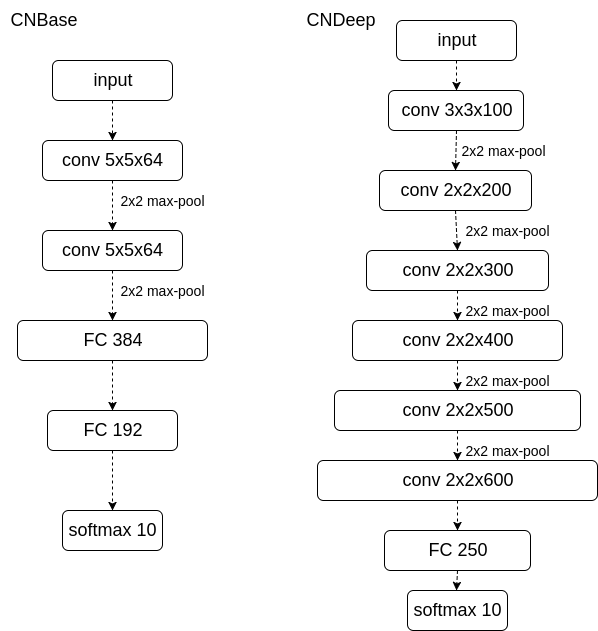
\includegraphics[width=0.45\textwidth]{models.png}}
\caption{The structure of two models: CNBase and CNDeep. ``FC 384'' represents a fully connected layer with 384 neurons etc.}
\label{fig1}
\end{figure}

\subsubsection*{CNFmp}
Applying fractional max pooling \cite{fmp} to CNDeep allowed stacking 13 convolutional layers, as in figure \ref{fig2}. Adding a final NiN layer made a total of 14 convolutional layers with a shape similar to $CN(32, 13)$. I shrinked the width factor $k$ to 32 so that the total number of parameters was controlled to 3.35 million. I used leaky ReLU with $\alpha=0.3$. Dropout rates increased linearly from $0.0$ to $0.2$.

\begin{figure}[htbp]
\centerline{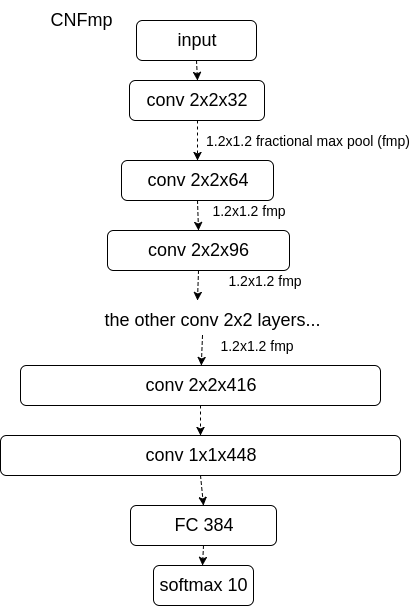
\includegraphics[width=0.3\textwidth]{fmp_model.png}}
\caption{The structure of CNFmp. It stacked 14 convolutional layers and 12 1.2x1.2 fractional max pooling operations.}
\label{fig2}
\end{figure}

\subsection*{Expriment Setup}
I implemented all the convolutional network models using Python 2.7 and Tensorflow. All the training and evaluation were running on my laptop with GPU 3GB GTX 770M.

I picked the GradientDescent Optimizer. I also tried other optimizers including Adam and Momentum, but coundn't get them to work, possibly due to proper parameter settings.

I set the learning rate to start with 0.1, which decayed exponentially after the first 10,000 steps. Approximately every 30,000 steps the learning rate was multiplied by a factor of 0.1. 

I adjusted the batch size to be 32 for training and 5 for evaluation. The max training step was set to 100,000. Higher batch size had led to crash due to running out of video memory.

In order to track the training state in real time, a checkpoint for the training model was saved every 2 minutes. A seperate process was running for evaluation on the test set, at the same time with the training process. The learner (training process) had no knowledge about the testing result.

\section{Results}
A short summary of my results can be found in table \ref{tab1}

\begin{table}[htbp]
\caption{Benchmark Summary}
\begin{center}
\begin{tabular}{|c|c|c|c|}
\hline
\textbf{Model}&\multicolumn{3}{|c|}{\textbf{Details}} \\
\cline{2-4} 
\textbf{Name} & \textbf{\textit{\#Parameters}}& \textbf{\textit{Test Accuracy \%}}& \textbf{\textit{Convergence Time}} \\
\hline
CNBase &1.76M  & 80.6& $>$ 55K steps, 3 hours\\
\hline
CNDeep & 2.96M & 85.6 & 55K steps, 2 hours \\
\hline
CNNiN & 4.14M & 85.5& 6K steps, 3 hours \\
\hline
CNFmp & 3.35M & 79.6 & 80K steps, 10 hours \\
\hline

\end{tabular}
\label{tab1}
\end{center}
\end{table}

\begin{figure}[htbp]
\centerline{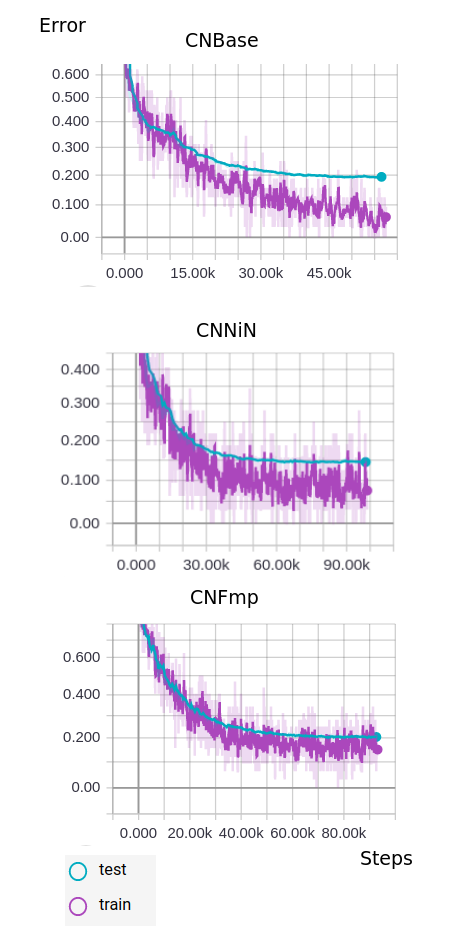
\includegraphics[width=0.45\textwidth]{result1.png}}
\caption{Training results of CNBase, CNNiN and CNFmp. Training and test errors vs steps. The error axes were log scaled. Visualization was done by Tensorboard.}
\label{fig3}
\end{figure}


\begin{table}[htbp]
\caption{CNDeep with Different Dropout Rates}
\begin{center}
\begin{tabular}{|c|c|c|}
\hline
\textbf{Max Drop Rate}& \textbf{\textit{Test Accuracy \%}}& \textbf{\textit{Convergence Time}} \\
\hline
0.0  & 85.6& 55K steps, 2 hours\\
\hline
0.2 & 85.3 & 70K steps, 3 hours \\
\hline
0.5 & 83.2& 100K steps, 4 hours \\
\hline
\end{tabular}
\label{tab2}
\end{center}
\end{table}

\begin{figure}[htbp]
\centerline{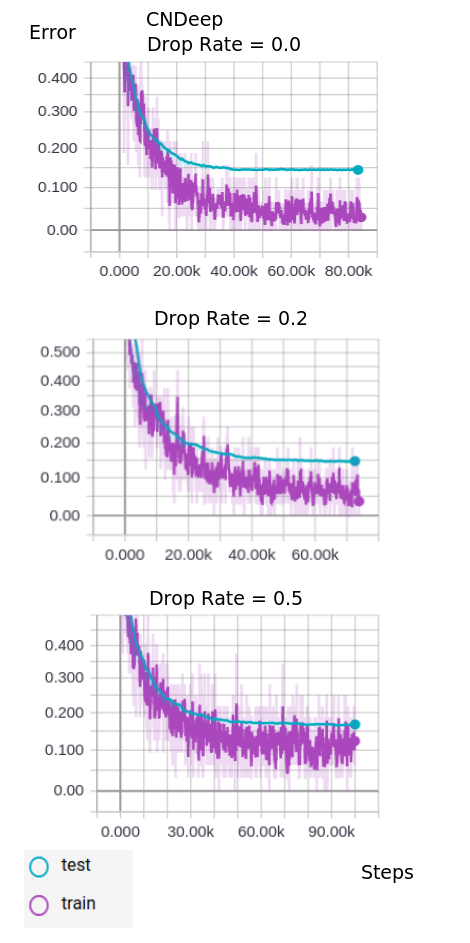
\includegraphics[width=0.45\textwidth]{result2.png}}
\caption{Training results of CNDeep with differet max dropout rates. The error axes were log scaled. Visualization was done by Tensorboard.}
\label{fig4}
\end{figure}

\section*{Acknowledgment}

placeholder


\FloatBarrier
\begin{thebibliography}{00}
\bibitem{cifar} Krizhevsky, Alex, and Geoffrey Hinton. ``Learning multiple layers of features from tiny images.'' (2009).
\bibitem{leaderboard} Rodrigo Benenson. ``Classification datasets results.'' \url{http://rodrigob.github.io/are_we_there_yet/build/classification_datasets_results.html}
\bibitem{conv}Krizhevsky, Alex, Ilya Sutskever, and Geoffrey E. Hinton. ``Imagenet classification with deep convolutional neural networks.'' Advances in neural information processing systems. 2012.
\bibitem{frac} Graham, Benjamin. ``Fractional max-pooling.'' arXiv preprint arXiv:1412.6071 (2014).
\bibitem{tut} ``Convolutional Neural Networks.'' \url{ https://www.tensorflow.org/tutorials/deep_cnn}
\bibitem{nin} Lin, Min, Qiang Chen, and Shuicheng Yan. ``Network in network.'' arXiv preprint arXiv:1312.4400 (2013).
\bibitem{sparse} Graham, Benjamin. ``Spatially-sparse convolutional neural networks.'' arXiv preprint arXiv:1409.6070 (2014).
\bibitem{fmp} Graham, Benjamin. ``Fractional max-pooling.'' arXiv preprint arXiv:1412.6071 (2014).
\bibitem{res} He, Kaiming, et al. ``Deep residual learning for image recognition.'' Proceedings of the IEEE conference on computer vision and pattern recognition. 2016.
\bibitem{wide} Zagoruyko, Sergey, and Nikos Komodakis. ``Wide residual networks.'' arXiv preprint arXiv:1605.07146 (2016).
\bibitem{cross} De Boer, Pieter-Tjerk, et al. ``A tutorial on the cross-entropy method.'' Annals of operations research 134.1 (2005): 19-67.
\bibitem{decay} Krogh, Anders, and John A. Hertz. "A simple weight decay can improve generalization." Advances in neural information processing systems. 1992.
\bibitem{leaky} Maas, Andrew L., Awni Y. Hannun, and Andrew Y. Ng. ``Rectifier nonlinearities improve neural network acoustic models.'' Proc. ICML. Vol. 30. No. 1. 2013.
\end{thebibliography}

\end{document}
